\section{Thuật toán Gradient trong định tuyến mạng}
\label{sec:gradient}

Trong các mạng cảm biến không dây và mạng ad-hoc, việc lựa chọn phương pháp định tuyến phù hợp đóng vai trò then chốt trong việc đảm bảo hiệu suất truyền thông và kéo dài tuổi thọ của mạng. Thuật toán định tuyến dựa trên Gradient (Gradient-based Routing) nổi lên như một giải pháp đơn giản nhưng hiệu quả, đặc biệt phù hợp với các mạng có tài nguyên hạn chế và topology thay đổi liên tục.

Phương pháp định tuyến Gradient mang lại nhiều ưu điểm đáng kể cho các ứng dụng mạng cảm biến và IoT:

\begin{itemize}
    \item Độ đơn giản trong triển khai: Mỗi node chỉ cần lưu trữ giá trị gradient của mình và thông tin về các node lân cận trực tiếp, giảm thiểu yêu cầu về bộ nhớ và khả năng tính toán.
    
    \item Overhead truyền thông thấp: Việc thiết lập và duy trì gradient chỉ yêu cầu các bản tin broadcast định kỳ từ sink node, không cần trao đổi thông tin định tuyến phức tạp giữa các node.
    
    \item Khả năng thích ứng với topology động: Khi có node mới tham gia hoặc rời khỏi mạng, gradient có thể được cập nhật cục bộ mà không ảnh hưởng đến hoạt động của toàn mạng.
    
    \item Khả năng tự phục hồi cao: Nếu đường truyền chính bị gián đoạn, node có thể nhanh chóng chuyển sang sử dụng đường truyền thay thế thông qua các node lân cận khác có gradient thấp hơn.
    
    \item Hỗ trợ tự nhiên cho định tuyến đa đường: Do có thể tồn tại nhiều node lân cận với gradient thấp hơn, thuật toán có thể khai thác nhiều đường đi song song để cân bằng tải hoặc tăng độ tin cậy, và tỷ lệ truyền tin thành công.
\end{itemize}

Những đặc điểm trên khiến thuật toán Gradient trở thành lựa chọn phù hợp cho các ứng dụng mạng cảm biến ad-hoc, đặc biệt trong bối cảnh các node có tài nguyên phần cứng hạn chế, cần tiết kiệm năng lượng và hoạt động trong môi trường với topology không ổn định. Các phần tiếp theo sẽ trình bày chi tiết về nguyên lý hoạt động, quá trình thiết lập gradient, cơ chế chuyển tiếp dữ liệu, cũng như các biến thể và cải tiến của thuật toán này.

\subsection{Nguyên lý hoạt động}

Ý tưởng cốt lõi của thuật toán Gradient bắt nguồn từ hiện tượng vật lý tự nhiên: dòng chảy của nước luôn di chuyển từ vùng có độ cao lớn xuống vùng có độ cao thấp hơn theo hướng gradient âm. Áp dụng nguyên lý này vào mạng truyền thông, mỗi node trong mạng được gán một giá trị số nguyên gọi là "gradient" (hay còn gọi là "độ cao logic"), biểu thị khoảng cách logic từ node đó đến sink node - điểm thu thập dữ liệu trung tâm của mạng. Sink node được gán giá trị gradient bằng 0, trong khi các node khác có giá trị gradient tăng dần theo số bước nhảy (hop count) cần thiết để đến được sink.

Khi một node cần truyền dữ liệu về sink, thay vì phải duy trì một bảng định tuyến phức tạp với thông tin về toàn bộ topology mạng, node chỉ cần thực hiện một quy tắc đơn giản: chuyển tiếp gói tin đến bất kỳ node lân cận nào có giá trị gradient thấp hơn giá trị gradient của chính nó. Quy tắc này đảm bảo rằng dữ liệu sẽ "chảy" một cách tự nhiên về phía sink node, giống như dòng nước chảy xuôi theo địa hình.

\begin{figure}[h!]
    \centering
    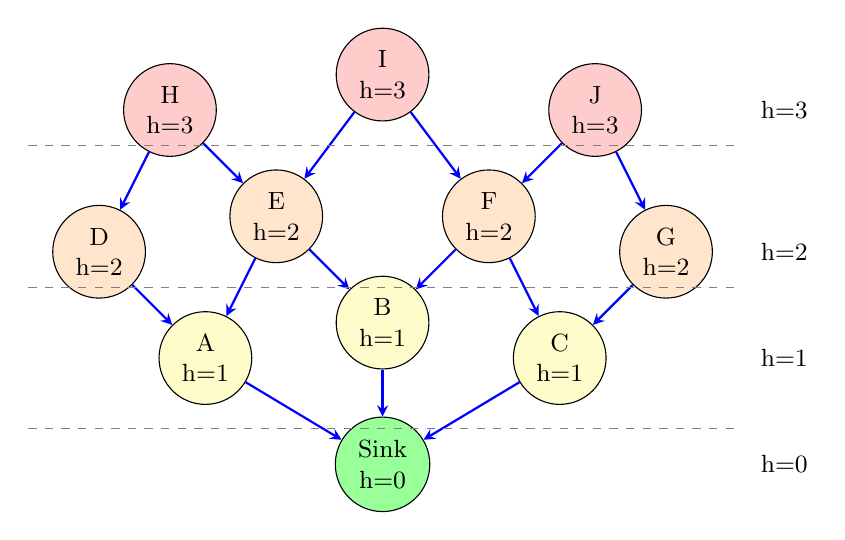
\begin{tikzpicture}[
        node/.style={circle, draw, minimum size=1cm, font=\small, align=center},
        sink/.style={circle, draw, fill=green!40, minimum size=1.2cm, font=\small, align=center},
        arrow/.style={->, >=stealth, thick, blue},
        scale=0.9
    ]
        % Sink node (height = 0)
        \node[sink] (Sink) at (0,0) {Sink\\h=0};
        
        % Level 1 nodes (height = 1)
        \node[node, fill=yellow!20] (A) at (-2.5,1.5) {A\\h=1};
        \node[node, fill=yellow!20] (B) at (0,2) {B\\h=1};
        \node[node, fill=yellow!20] (C) at (2.5,1.5) {C\\h=1};
        
        % Level 2 nodes (height = 2)
        \node[node, fill=orange!20] (D) at (-4,3) {D\\h=2};
        \node[node, fill=orange!20] (E) at (-1.5,3.5) {E\\h=2};
        \node[node, fill=orange!20] (F) at (1.5,3.5) {F\\h=2};
        \node[node, fill=orange!20] (G) at (4,3) {G\\h=2};
        
        % Level 3 nodes (height = 3)
        \node[node, fill=red!20] (H) at (-3,5) {H\\h=3};
        \node[node, fill=red!20] (I) at (0,5.5) {I\\h=3};
        \node[node, fill=red!20] (J) at (3,5) {J\\h=3};
        
        % Gradient arrows (data flow direction)
        \draw[arrow] (A) -- (Sink);
        \draw[arrow] (B) -- (Sink);
        \draw[arrow] (C) -- (Sink);
        
        \draw[arrow] (D) -- (A);
        \draw[arrow] (E) -- (A);
        \draw[arrow] (E) -- (B);
        \draw[arrow] (F) -- (B);
        \draw[arrow] (F) -- (C);
        \draw[arrow] (G) -- (C);
        
        \draw[arrow] (H) -- (D);
        \draw[arrow] (H) -- (E);
        \draw[arrow] (I) -- (E);
        \draw[arrow] (I) -- (F);
        \draw[arrow] (J) -- (F);
        \draw[arrow] (J) -- (G);
        
        % Height levels indication
        \draw[dashed, gray] (-5,0.5) -- (5,0.5);
        \draw[dashed, gray] (-5,2.5) -- (5,2.5);
        \draw[dashed, gray] (-5,4.5) -- (5,4.5);
        
        \node[right] at (5.2,0) {\small h=0};
        \node[right] at (5.2,1.5) {\small h=1};
        \node[right] at (5.2,3) {\small h=2};
        \node[right] at (5.2,5) {\small h=3};
    \end{tikzpicture}
    \caption{Minh họa nguyên lý định tuyến Gradient với giá trị độ cao (height)}
    \label{fig:gradient_principle}
\end{figure}

Hình \ref{fig:gradient_principle} minh họa nguyên lý hoạt động của thuật toán Gradient. Sink node có giá trị Gradient = 0, các node lân cận trực tiếp có Gradient = 1, và Gradient tăng dần theo số hop. Mũi tên màu xanh thể hiện hướng chuyển tiếp dữ liệu, luôn đi từ node có Gradient lớn hơn đến node có Gradient nhỏ hơn.

\subsection{Quá trình thiết lập Gradient}

Quá trình thiết lập gradient trong mạng được thực hiện thông qua cơ chế phát tán thông tin từ sink node. Quá trình này bao gồm các bước sau:

\textbf{Bước 1: Khởi tạo từ Sink node.} Sink node khởi tạo quá trình bằng cách broadcast một gói tin Interest (hoặc Advertisement) chứa thông tin về độ cao của nó (Gradient=0) và một số thứ tự (sequence number) để đảm bảo tính mới của thông tin.

\textbf{Bước 2: Lan truyền và cập nhật độ cao.} Khi một node nhận được gói tin Interest từ node lân cận với độ cao $Gradient_{neighbor}$, nó sẽ:
\begin{itemize}
    \item Kiểm tra số thứ tự để đảm bảo thông tin mới hơn thông tin hiện có
    \item Cập nhật độ cao của mình: $Gradient_{self} = Gradient_{neighbor} + 1$
    \item Ghi nhận node gửi là "node cha" tiềm năng (parent node) để chuyển tiếp dữ liệu
    \item Broadcast gói tin Interest với độ cao mới đến các node lân cận khác
\end{itemize}

\textbf{Bước 3: Hội tụ.} Quá trình tiếp tục cho đến khi tất cả các node trong mạng đã nhận được thông tin và thiết lập được giá trị độ cao. Sau khi hội tụ, mỗi node biết được khoảng cách logic của mình đến sink và có ít nhất một node lân cận với độ cao thấp hơn để chuyển tiếp dữ liệu.

\begin{figure}[h!]
    \centering
    \begin{tikzpicture}[
        node/.style={circle, draw, minimum size=0.7cm, font=\scriptsize, align=center},
        sink/.style={circle, draw, fill=green!40, minimum size=0.8cm, font=\scriptsize, align=center},
        packet/.style={->, >=stealth, thick, red, dashed},
        scale=0.75
    ]
        % === Step 1 ===
        \node at (-6, 4) {\textbf{Bước 1}};
        \node[sink] (S1) at (-6,2.5) {Sink\\h=0};
        \node[node] (A1) at (-7.5,1) {A\\h=?};
        \node[node] (B1) at (-6,0.5) {B\\h=?};
        \node[node] (C1) at (-4.5,1) {C\\h=?};
        \draw (S1) -- (A1); \draw (S1) -- (B1); \draw (S1) -- (C1);
        \draw[packet] (S1) -- (A1); \draw[packet] (S1) -- (B1); \draw[packet] (S1) -- (C1);
        \node at (-6,-0.8) {\scriptsize Sink broadcast};
        
        % === Step 2 ===
        \node at (0, 4) {\textbf{Bước 2}};
        \node[sink] (S2) at (0,2.5) {Sink\\h=0};
        \node[node, fill=yellow!20] (A2) at (-1.5,1) {A\\h=1};
        \node[node, fill=yellow!20] (B2) at (0,0.5) {B\\h=1};
        \node[node, fill=yellow!20] (C2) at (1.5,1) {C\\h=1};
        \node[node] (D2) at (-1.5,-1) {D\\h=?};
        \node[node] (E2) at (1.5,-1) {E\\h=?};
        \draw (S2) -- (A2); \draw (S2) -- (B2); \draw (S2) -- (C2);
        \draw (A2) -- (D2); \draw (C2) -- (E2); \draw (B2) -- (D2); \draw (B2) -- (E2);
        \draw[packet] (A2) -- (D2); \draw[packet] (B2) -- (D2);
        \draw[packet] (C2) -- (E2); \draw[packet] (B2) -- (E2);
        \node at (0,-2.2) {\scriptsize Node h=1 broadcast};
        
        % === Step 3 ===
        \node at (6, 4) {\textbf{Bước 3 (Hội tụ)}};
        \node[sink] (S3) at (6,2.5) {Sink\\h=0};
        \node[node, fill=yellow!20] (A3) at (4.5,1) {A\\h=1};
        \node[node, fill=yellow!20] (B3) at (6,0.5) {B\\h=1};
        \node[node, fill=yellow!20] (C3) at (7.5,1) {C\\h=1};
        \node[node, fill=orange!20] (D3) at (4.5,-1) {D\\h=2};
        \node[node, fill=orange!20] (E3) at (7.5,-1) {E\\h=2};
        \draw (S3) -- (A3); \draw (S3) -- (B3); \draw (S3) -- (C3);
        \draw (A3) -- (D3); \draw (C3) -- (E3); \draw (B3) -- (D3); \draw (B3) -- (E3);
        \node at (6,-2.2) {\scriptsize Gradient thiết lập xong};
    \end{tikzpicture}
    \caption{Quá trình thiết lập Gradient trong mạng}
    \label{fig:gradient_setup}
\end{figure}

\subsection{Quá trình chuyển tiếp dữ liệu}

Sau khi gradient được thiết lập, quá trình chuyển tiếp dữ liệu từ node nguồn đến sink diễn ra như sau:

\begin{enumerate}
    \item Node nguồn có dữ liệu cần gửi sẽ tìm trong danh sách các node lân cận những node có độ cao thấp hơn độ cao của mình.
    \item Node nguồn chọn một hoặc nhiều node lân cận có độ cao thấp hơn để chuyển tiếp dữ liệu. Việc chọn có thể dựa trên các tiêu chí như: node có độ cao thấp nhất, node có chất lượng liên kết tốt nhất, hoặc node có năng lượng còn lại cao nhất.
    \item Node nhận được dữ liệu tiếp tục quá trình tương tự, chuyển tiếp đến node có độ cao thấp hơn.
    \item Quá trình lặp lại cho đến khi dữ liệu đến được sink node (Gradient=0).
\end{enumerate}

Thuật toán chuyển tiếp dữ liệu có thể được mô tả như sau:

\begin{center}
\small
\fbox{\parbox{0.85\textwidth}{
\textbf{Thuật toán: Chuyển tiếp dữ liệu dựa trên Gradient}

\textbf{Đầu vào:} Gói tin $P$, Gradient hiện tại $G_{self}$, Danh sách lân cận $N$

\textbf{Đầu ra:} Chuyển tiếp $P$ đến sink node

\vspace{0.5em}
\begin{tabular}{@{}ll@{}}
1. & \textbf{Nếu} $G_{self} = 0$ \textbf{thì} xử lý $P$ (đã đến sink), \textbf{kết thúc} \\
2. & Khởi tạo tập ứng viên $C \gets \emptyset$ \\
3. & \textbf{Với mỗi} $n \in N$: \textbf{nếu} $G_n < G_{self}$ \textbf{thì} $C \gets C \cup \{n\}$ \\
4. & \textbf{Nếu} $C = \emptyset$ \textbf{thì} hủy gói tin hoặc lưu tạm, \textbf{kết thúc} \\
5. & $next\_hop \gets \text{selectBest}(C)$; Gửi $P$ đến $next\_hop$ \\
\end{tabular}
}}
\end{center}

\subsection{Cơ chế duy trì và cập nhật Gradient}

Trong mạng ad-hoc với topology động, gradient cần được cập nhật khi có sự thay đổi trong mạng. Có hai cơ chế chính để duy trì gradient:

Cập nhật định kỳ: Tất cả các node định kỳ broadcast thông tin về Gradient của mình đến các node lân cận để làm mới thông tin gradient trong toàn mạng. Phương pháp này đơn giản nhưng gây overhead đều đặn.

Cập nhật theo sự kiện: Node sẽ broadcast thông tin về Gradient của mình đến tất cả các node lân cận khi có sự thay đổi cấu trúc mạng xung quanh node đó, ví dụ:
\begin{itemize}
    \item Khi một node mất kết nối với tất cả các node có độ cao thấp hơn
    \item Khi phát hiện node mới tham gia mạng
    \item Khi chất lượng liên kết thay đổi đáng kể
\end{itemize}

\begin{figure}[h!]
    \centering
    \begin{tikzpicture}[
        node/.style={circle, draw, minimum size=0.9cm, font=\scriptsize, align=center},
        sink/.style={circle, draw, fill=green!40, minimum size=1cm, font=\scriptsize, align=center},
        failed/.style={circle, draw, fill=red!40, minimum size=0.9cm, font=\scriptsize, dashed, align=center},
        arrow/.style={->, >=stealth, thick, blue},
        newarrow/.style={->, >=stealth, thick, orange, dashed},
        scale=0.85
    ]
        % === Before failure ===
        \node at (-4, 4) {\textbf{(a) Trước khi node B hỏng}};
        
        \node[sink] (S1) at (-4,2.5) {Sink\\h=0};
        \node[node, fill=yellow!20] (A1) at (-5.5,1.5) {A\\h=1};
        \node[node, fill=yellow!20] (B1) at (-4,1) {B\\h=1};
        \node[node, fill=yellow!20] (C1) at (-2.5,1.5) {C\\h=1};
        \node[node, fill=orange!20] (D1) at (-4,-0.5) {D\\h=2};
        
        \draw (S1) -- (A1); \draw (S1) -- (B1); \draw (S1) -- (C1);
        \draw (B1) -- (D1); \draw (A1) -- (D1); \draw (C1) -- (D1);
        \draw[arrow] (D1) -- (B1);
        \draw[arrow] (B1) -- (S1);
        
        % === After failure ===
        \node at (4, 4) {\textbf{(b) Sau khi node B hỏng}};
        
        \node[sink] (S2) at (4,2.5) {Sink\\h=0};
        \node[node, fill=yellow!20] (A2) at (2.5,1.5) {A\\h=1};
        \node[failed] (B2) at (4,1) {B\\h=1};
        \node[node, fill=yellow!20] (C2) at (5.5,1.5) {C\\h=1};
        \node[node, fill=orange!20] (D2) at (4,-0.5) {D\\h=2};
        
        \draw (S2) -- (A2); \draw[dashed, gray] (S2) -- (B2); \draw (S2) -- (C2);
        \draw[dashed, gray] (B2) -- (D2); \draw (A2) -- (D2); \draw (C2) -- (D2);
        \draw[newarrow] (D2) -- (A2);
        \draw[arrow] (A2) -- (S2);
        
        \node at (4,-1.8) {\scriptsize D chuyển sang dùng A làm next-hop};
    \end{tikzpicture}
    \caption{Khả năng phục hồi của thuật toán Gradient khi có node hỏng}
    \label{fig:gradient_recovery}
\end{figure}

Hình \ref{fig:gradient_recovery} minh họa khả năng phục hồi của thuật toán Gradient. Khi node B hỏng, node D vẫn có thể chuyển tiếp dữ liệu thông qua node A hoặc C vì cả hai đều có độ cao thấp hơn D. Đây là một trong những ưu điểm quan trọng của thuật toán Gradient: khả năng tự phục hồi mà không cần tính toán lại toàn bộ đường đi.

\subsection{Các biến thể của thuật toán Gradient}

\subsubsection{Gradient với đa metric}

Ngoài việc sử dụng số hop làm metric duy nhất, Gradient có thể được tính dựa trên nhiều yếu tố kết hợp giúp cải thiện chất lượng của đường đi. Ví dụ, một hàm gradient tổng hợp có thể được định nghĩa như sau:

\begin{equation}
    h_{combined} = \alpha \cdot h_{hop} + \beta \cdot h_{energy} + \gamma \cdot h_{quality}
    \label{eq:multi_metric_gradient}
\end{equation}

Trong đó:
\begin{itemize}
    \item $h_{hop}$: Số hop đến sink
    \item $h_{energy}$: Hệ số liên quan đến năng lượng còn lại (node năng lượng thấp có $h_{energy}$ cao hơn)
    \item $h_{quality}$: Hệ số liên quan đến chất lượng liên kết
    \item $\alpha, \beta, \gamma$: Trọng số của các yếu tố
\end{itemize}

Việc có thêm tham số liên quan đến năng lượng giúp kéo dài tuổi thọ mạng bằng cách tránh sử dụng quá mức các node có năng lượng thấp. Ngoài ra, việc đưa các giá trị này vào hàm gradient giúp tính toán được chất lượng của cả đường đi từ node đó về sink node.

\subsubsection{Gradient với cân bằng tải}

Để tránh tình trạng một số node bị quá tải do nằm trên đường đi chính, thuật toán có thể sử dụng cơ chế chọn ngẫu nhiên có trọng số giữa các node lân cận có độ cao thấp hơn:

\begin{equation}
    P(n) = \frac{w_n}{\sum_{i \in candidates} w_i}
    \label{eq:load_balance}
\end{equation}

Trong đó $w_n$ là trọng số của node $n$, có thể dựa trên năng lượng còn lại, số gói tin đang chờ xử lý, hoặc chất lượng liên kết.

\subsection{Ưu điểm và nhược điểm}

\textbf{Ưu điểm:}
\begin{itemize}
    \item Đơn giản: Mỗi node chỉ cần lưu trữ độ cao của mình và thông tin về các node lân cận, không cần bảng định tuyến phức tạp.
    \item Overhead thấp: Chỉ cần broadcast gói tin Interest khi thiết lập hoặc cập nhật gradient, không cần trao đổi thông tin định tuyến liên tục.
    \item Khả năng mở rộng tốt: Phù hợp với mạng có số lượng node lớn vì mỗi node chỉ cần thông tin cục bộ.
    \item Khả năng phục hồi cao: Khi một đường đi bị hỏng, node có thể nhanh chóng chuyển sang sử dụng node lân cận khác có độ cao thấp hơn.
    \item Hỗ trợ đa đường: Tự nhiên hỗ trợ nhiều đường đi đến sink, có thể khai thác để cân bằng tải hoặc tăng độ tin cậy.
    \item Khả năng phát triển thêm: Dễ dàng tích hợp các yếu tố khác như năng lượng, chất lượng liên kết vào hàm gradient để cải thiện hiệu suất định tuyến. 
\end{itemize}

\textbf{Nhược điểm:}
\begin{itemize}
    \item Không tối ưu cho mọi trường hợp: Đường đi theo gradient không phải lúc nào cũng là đường đi ngắn nhất hoặc tốt nhất về mặt năng lượng.
    \item Vấn đề với mạng thưa: Trong mạng có mật độ node thấp, có thể xảy ra tình trạng "hố đen" (void) khi một node không có node lân cận nào có độ cao thấp hơn.
    \item Phụ thuộc vào sink: Gradient được thiết lập từ sink, nên không phù hợp với các ứng dụng yêu cầu truyền thông peer-to-peer giữa các node bất kỳ.
\end{itemize}

\subsection{So sánh với các phương pháp định tuyến khác}

Bảng \ref{tab:gradient_comparison} so sánh thuật toán Gradient với các phương pháp định tuyến phổ biến khác trong mạng cảm biến.

\begin{table}[h!]
\centering
\caption{So sánh thuật toán Gradient với các phương pháp định tuyến khác}
\label{tab:gradient_comparison}
\begin{tabular}{|l|c|c|c|c|}
\hline
\textbf{Tiêu chí} & \textbf{Flooding} & \textbf{AODV} & \textbf{LEACH} & \textbf{Gradient} \\
\hline
Overhead thiết lập & Không & Cao & Trung bình & Thấp \\
\hline
Overhead duy trì & Rất cao & Thấp & Trung bình & Thấp \\
\hline
Độ trễ & Thấp & Cao & Trung bình & Thấp \\
\hline
Tiêu thụ năng lượng & Rất cao & Trung bình & Thấp & Thấp \\
\hline
Khả năng mở rộng & Thấp & Trung bình & Cao & Cao \\
\hline
Độ tin cậy & Cao & Trung bình & Trung bình & Cao \\
\hline
Độ phức tạp & Rất thấp & Cao & Trung bình & Thấp \\
\hline
\end{tabular}
\end{table}

% ...existing code...

Từ bảng so sánh có thể thấy thuật toán Gradient có sự cân bằng tốt giữa các yếu tố: overhead thấp, độ trễ thấp, tiêu thụ năng lượng thấp và khả năng mở rộng cao. Đây là những đặc điểm phù hợp với yêu cầu của mạng cảm biến ad-hoc trong các ứng dụng IoT, nơi các node có tài nguyên hạn chế và cần hoạt động trong thời gian dài.

Cụ thể hơn, khi so sánh với phương pháp Flooding - một trong những phương pháp đơn giản nhất, thuật toán Gradient vượt trội hoàn toàn về mặt tiêu thụ năng lượng và overhead duy trì. Trong khi Flooding làm cho mỗi gói tin được broadcast đến tất cả các node trong mạng, gây ra tiêu tốn năng lượng rất lớn, thuật toán Gradient chỉ chuyển tiếp gói tin theo một hướng xác định - hướng về phía sink node. Điều này giúp giảm đáng kể số lượng bản tin truyền trong mạng.

So với AODV (Ad-hoc On-demand Distance Vector) - một giao thức định tuyến reactive phổ biến trong mạng ad-hoc, thuật toán Gradient có ưu thế về độ trễ và overhead thiết lập. AODV yêu cầu quá trình route discovery mỗi khi cần truyền dữ liệu đến một đích mới, bao gồm việc broadcast gói Route Request (RREQ) và chờ đợi gói Route Reply (RREP). Quá trình này gây ra độ trễ đáng kể, đặc biệt trong các mạng lớn. Ngược lại, thuật toán Gradient thiết lập sẵn gradient từ trước, cho phép node bắt đầu truyền dữ liệu ngay lập tức mà không cần chờ đợi quá trình khám phá đường đi.

Khi so sánh với LEACH (Low-Energy Adaptive Clustering Hierarchy) - một giao thức phân cụm được thiết kế đặc biệt cho mạng cảm biến, thuật toán Gradient có độ phức tạp triển khai thấp hơn và không yêu cầu cơ chế bầu chọn cluster head phức tạp. LEACH phân chia mạng thành các cụm với một node đóng vai trò cluster head chịu trách nhiệm thu thập và tổng hợp dữ liệu từ các node thành viên. Mặc dù cách tiếp cận này hiệu quả về mặt năng lượng trong một số trường hợp, nó đòi hỏi các giai đoạn setup định kỳ để bầu chọn lại cluster head, gây ra overhead và độ trễ. Thuật toán Gradient không có khái niệm về cluster head, mỗi node đều bình đẳng và có thể tham gia vào quá trình chuyển tiếp dữ liệu.

Một điểm mạnh quan trọng của thuật toán Gradient là khả năng hỗ trợ tự nhiên cho định tuyến đa đường (multipath routing). Do mỗi node có thể có nhiều node lân cận với giá trị gradient thấp hơn, dữ liệu có thể được chuyển tiếp qua nhiều đường đi khác nhau. Đặc điểm này mang lại hai lợi ích quan trọng: thứ nhất, nó tăng độ tin cậy của việc truyền dữ liệu vì nếu một đường đi bị gián đoạn, dữ liệu vẫn có thể đến được sink thông qua đường đi khác; thứ hai, nó cho phép cân bằng tải giữa các node, tránh tình trạng một số node bị quá tải trong khi các node khác nhàn rỗi.

Bên cạnh đó, thuật toán Gradient còn có khả năng tích hợp dễ dàng với các cơ chế khác để cải thiện hiệu suất. Ví dụ, giá trị gradient có thể được kết hợp với thông tin về năng lượng còn lại của node để tối ưu hóa tuổi thọ mạng, hoặc kết hợp với chỉ số chất lượng liên kết (Link Quality Indicator - LQI) để tăng độ tin cậy truyền tin. Tính linh hoạt này làm cho thuật toán Gradient trở thành một nền tảng vững chắc để xây dựng các giải pháp định tuyến phức tạp hơn.

Tổng kết lại, thuật toán Gradient nổi bật với sự đơn giản trong thiết kế, hiệu quả trong hoạt động, và khả năng thích ứng với các yêu cầu đa dạng của mạng cảm biến ad-hoc. Những đặc điểm này khiến nó trở thành lựa chọn phù hợp cho việc triển khai trên các nền tảng phần cứng có tài nguyên hạn chế như vi điều khiển nRF54L15 của Nordic Semiconductor, nơi mà sự tiết kiệm bộ nhớ, năng lượng và khả năng xử lý là các yếu tố then chốt quyết định tính khả thi của giải pháp.
